\documentclass{beamer}

\useoutertheme[subsection=false]{miniframes}
\usecolortheme{beaver}
\setbeamertemplate{navigation symbols}{}
\setbeamertemplate{footline}{}
\usepackage{graphicx}
\usepackage{url}
\usepackage{datetime}
\usepackage{tikz-cd}
\newcommand{\lectureDate}{\formatdate{01}{11}{2018}}

\setbeamertemplate{caption}
{\raggedright\insertcaption\par}
\title{MATH211: Linear Methods I}
\author{Matthew Burke}
\date{\lectureDate}
\begin{document}

\frame{\titlepage}

\begin{frame}{Lecture on \lectureDate}
  \tableofcontents
\end{frame}

\section*{Last time}
\label{sec:Last-time}

\begin{frame}{Last time}
  \begin{itemize}
  \item Linear transformations\vfill
  \item Action on compositions\vfill
  \item Matrix of a linear transformation
  \end{itemize}
\end{frame}

\section{Matrices}

\begin{frame}
\begin{beamercolorbox}[sep=12pt,center]{part title}
\usebeamerfont{section title}
\insertsection\par
\end{beamercolorbox}
\end{frame}

\begin{frame}{Matrices and linear transformations}
\begin{example}
If $A$ is an $m\times n$ matrix then the function $x\mapsto Ax$ is a linear transformation $\mathbb{R}^n \rightarrow \mathbb{R}^m$.
\end{example}\vfill
\begin{definition}
If \(T:\mathbb{R}^n \rightarrow \mathbb{R}^m\) is a linear transformation then the \emph{matrix $[T]$ of $T$} has columns given by the images of the standard basis vectors:
\begin{equation*}
[T] = \left[
\begin{array}{cccc}
T(e_1) & T(e_2) &\dots & T(e_n)
\end{array}
\right]
\end{equation*} 
\end{definition}
\end{frame}

\begin{frame}{Examples}
\begin{example}
What is the matrix of the linear transformation for counter-clockwise rotation about the origin by an angle of $\theta$?
\end{example}
\begin{example}
What is the matrix of the linear transformation for reflection in the line through that origin at an angle $\theta$ from the $x$-axis?
\end{example}
\begin{example}
What is the matrix of the linear transformation that is $v\times (-)$ for some vector $v\in \mathbb{R}^3$?
\end{example}
\end{frame}

\section{Composition}

\begin{frame}
\begin{beamercolorbox}[sep=12pt,center]{part title}
\usebeamerfont{section title}
\insertsection\par
\end{beamercolorbox}
\end{frame}

\begin{frame}{Composition of functions}
\begin{definition}
If we have functions
\begin{equation*}
\mathbb{R}^n \xrightarrow{f} \mathbb{R}^m \text{ and }\mathbb{R}^m \xrightarrow{g} \mathbb{R}^p
\end{equation*}
then the \emph{composite function $g\circ f$} is the function defined by
\begin{equation*}
(g\circ f)(x) = g(f(x))
\end{equation*}
\end{definition}
\begin{itemize}
	\item I.e. first apply $f$ to $x$ and then apply $g$ to the result.
	\item Note that $\mathbb{R}^n \xrightarrow{g\circ f} \mathbb{R}^p$.
\end{itemize}
\end{frame}

\begin{frame}{Composite of linear transformations}
\begin{example}
The composite of two linear transformations is again linear.
\begin{proof}
Suppose that $S:\mathbb{R}^m \rightarrow \mathbb{R}^p$ and $T:\mathbb{R}^n \rightarrow \mathbb{R}^m$ are linear transformations. Then
\begin{align*}
(S\circ T)(x+y) &= S(T(x+y)) = S(T(x)+T(y)) \\
&= S(T(x)) + S(T(y)) = (S\circ T)(x) + (S\circ T)(y)
\end{align*}
and
\begin{align*}
(S\circ T)(kx) &= S(T(kx)) = S(kT(x))\\
&= kS(T(x)) = k(S\circ T)(x)
\end{align*}
\end{proof}
\end{example}
\end{frame}

\begin{frame}{Matrix of composite transformation}
We know that the matrix of the composite $T\circ S$ is:
\begin{equation*}
\left[
\begin{array}{cccc}
T(S(e_1)) & T(S(e_2)) & \dots & T(S(e_n))
\end{array}
\right]
\end{equation*}
where $S: \mathbb{R}^n \rightarrow \mathbb{R}^m$ and $T: \mathbb{R}^m \rightarrow \mathbb{R}^p$.\vfill
\begin{theorem}
The matrix of a composite is the composite of the matrices:
\begin{equation*}
[T\circ S] = [T][S]
\end{equation*}
\begin{proof}
Note that the terms $S(e_i)$ are the columns of $[S]$.
\end{proof}
\end{theorem}

\end{frame}

\begin{frame}{Determinant of rotations and reflections}
\begin{example}[Determinant of rotation]
\begin{align*}
\left|
\begin{array}{cc}
\cos\theta & -\sin\theta\\
\sin\theta & \cos\theta
\end{array}
\right| = \cos^2\theta + \sin^2\theta = 1
\end{align*}
\end{example}
\begin{example}[Determinant of reflection]
\[\left|
\begin{array}{cc}
\cos\theta & \sin\theta\\
\sin\theta & -\cos\theta
\end{array}
\right|  = -\sin^2\theta -\cos^2\theta = -1
\]
\end{example}
\end{frame}

\begin{frame}{Composites of rotations and reflections}
In general,
\begin{itemize}
\item The composite of two rotations is a rotation
\[
R_\theta\circ R_\eta=R_{\theta+\eta}
\]
\item The composite of two reflections is a rotation.
\[
Q_m\circ Q_n = R_{\theta}
\]
where $\theta$ is $2\times$ the  angle between lines $y=mx$ and $y=nx$. 
\bigskip
\item The composite of a reflection and a rotation is a 
reflection.
\[
R_{\theta}\circ Q_n
= 
Q_m\circ Q_n\circ Q_n  
=Q_m
\]
\end{itemize}
\end{frame}


\begin{frame}{Examples}
\begin{example}
What is the matrix of the linear transformation that is the composite of reflection in the x-axis followed by rotation through an angle of $\frac{\pi}{2}$?
\end{example}
\begin{example}
What is the matrix of the linear transformation that is the composite of reflection in the line $y = -x$ followed by reflection in the y-axis.
\end{example}
\begin{example}
If
\begin{equation*}
S \left[
\begin{array}{c}
x\\
y
\end{array}
\right] = \left[
\begin{array}{c}
x\\
-y
\end{array}
\right]\text{ and } T \left[
\begin{array}{c}
x\\
y
\end{array}
\right] = \left[
\begin{array}{c}
-y\\
x
\end{array}
\right]
\end{equation*}
then find $S\circ T$, $T\circ S$ and the matrices $[S\circ T]$ and $[T\circ S]$.
\end{example}
\end{frame}

\section{Inverses}

\begin{frame}
\begin{beamercolorbox}[sep=12pt,center]{part title}
\usebeamerfont{section title}
\insertsection\par
\end{beamercolorbox}
\end{frame}

\begin{frame}{Inverse functions}
\begin{definition}[Identity transformation]
The \emph{identity transformation on $\mathbb{R}^n$} is the function $\mathbb{R}^n \rightarrow \mathbb{R}^n$ defined by $x\mapsto x$.
\end{definition}
\begin{definition}
If $S,T:\mathbb{R}^n \rightarrow \mathbb{R}^n$ are linear transformations then $S$ is inverse to $T$ iff 
\begin{equation*}
(S\circ T) = id = (T\circ S)
\end{equation*}
and we write $S = T^{-1}$ and $T = S^{-1}$.
\end{definition}
\begin{theorem}
If $[S]$ is the matrix of $S$ and $[T]$ is the matrix of $T$ then:
\begin{equation*}
S^{-1} = T \iff [S]^{-1} = [T]
\end{equation*}
\end{theorem}
\end{frame}

\begin{frame}{Examples}
\begin{example}
If
\begin{equation*}
T \left[
\begin{array}{c}
x\\
y
\end{array}
\right] = \left[
\begin{array}{c}
x+y\\
y
\end{array}
\right]
\end{equation*}
find $T^{-1}$ and $[T^{-1}]$.
\end{example}
\begin{example}
In general, what is the inverse of the linear transformation
\begin{equation*}
T \left[
\begin{array}{c}
x\\
y
\end{array}
\right] = \left[
\begin{array}{c}
ax +by\\
cx+dy
\end{array}
\right]
\end{equation*}
\end{example}
\end{frame}


\section{Complex numbers}

\begin{frame}
\begin{beamercolorbox}[sep=12pt,center]{part title}
\usebeamerfont{section title}
\insertsection\par
\end{beamercolorbox}
\end{frame}

\begin{frame}{Progression of thought about complex numbers}

% \begin{quote}
% .. subtle as they are useless ..
% \end{quote}
% (Girolamo Cardano - discoverer of complex numbers)
% \vfill
\begin{quote}
\dots the whole matter seems to rest on sophistry rather than truth\dots
\end{quote}
(Rafael Bombelli 1526-1572. Early innovator in use of complex numbers)
\vfill
\begin{quote}
The shortest path between two truths in the real domain passes through the complex domain.
\end{quote}
(Jacques Hadamard 1865-1963)
% \begin{quote}
% Indeed, nowadays no electrical engineer could get along without complex numbers, and neither could anyone working in aerodynamics or fluid dynamics.
% \end{quote}
% (Keith Devlin - British mathematician)

% \vfill

% \begin{quote}
% The imaginary number is a fine and wonderful resource of the human spirit, almost an amphibian between being and not being.
% \end{quote}
% (Leibniz)
\end{frame}

% \begin{frame}{More recently...}
% \begin{quote}
% It has been written that the shortest and best way between two truths of the real domain often passes through the imaginary one.
% \end{quote}
% (Jacques Hadamard)
% \vfill

% \begin{quote}
% I tell you, with complex numbers you can do anything.
% \end{quote}
% (John Derbyshire - mathematics writer)
% \vfill

% \begin{quote}
% Indeed, nowadays no electrical engineer could get along without complex numbers, and neither could anyone working in aerodynamics or fluid dynamics.
% \end{quote}
% (Keith Devlin - British mathematician)
% \end{frame}

\begin{frame}{Algebraic motivation - extending the number system}
\begin{quote}
God made the integers; all else is the work of man.
\end{quote}
(Leopold Kronecker)\vfill
\begin{itemize}
	\item Using only positive integers $\{1, 2, 3, \dots\}$
	\begin{itemize}
		\item we cannot find solution a to $x+1 = 0$
	\end{itemize}\vfill
	\item Using only integers $\{\dots, -2, -1, 0, 1, 2 \dots\}$
	\begin{itemize}
		\item we cannot find a solution to $3x+2 = 0$
	\end{itemize}\vfill
	\item Using only fractions $\{\frac{a}{b} \text{ for } b\neq0 \}$
	\begin{itemize}
		\item we cannot find a solution to $x^2-2 =0$
	\end{itemize}\vfill
	\item Using only decimals
	\begin{itemize}
		\item we cannot find a solution to $x^2 + 1 = 0$\dots
	\end{itemize}
\end{itemize}
\end{frame}

\begin{frame}{Complex numbers}
\begin{definition}
\begin{itemize}
\item
The \emph{imaginary unit}, denoted $i$, is defined to be
a number with the property that $i^2=-1$.
\item
A \emph{pure imaginary} number has the form $bi$ where 
$b\in \mathbb{R}$, $b\neq 0$.
\item
A \emph{complex number} is any number $z$ of the form
\[ z = a + bi\]
where $a,b\in \mathbb{R}$ and $i$ is the imaginary unit.
\end{itemize}
\end{definition}
\begin{definition}
If $z = a + bi$ then:
\begin{itemize}
\item
$a$ is called the \emph{real part} of $z$.
\item
$b$ is called the \emph{imaginary part} of $z$.
\end{itemize}
\end{definition}
\end{frame}

\begin{frame}[fragile]{Graphical interpretation}
Consider the function $\mathbb{R} \rightarrow \mathbb{R}$ that multiplies by $-1$:
\begin{equation*}
\begin{tikzcd}
-3\arrow[bend left, color = blue]{rrrrrr} & -2\arrow[bend left, color = blue]{rrrr} & -1 \arrow[bend left, color = blue]{rr} & 0 & +1\arrow[bend left, color = blue]{ll} & +2\arrow[bend left, color = blue]{llll} & +3\arrow[bend left, color = blue]{llllll}\\
\end{tikzcd}
\end{equation*}
which shows us that $-1\times(-1\times x) = x$.
\end{frame}

\begin{frame}[fragile]{Graphical interpretation}
So how do we get a transformation that squares to $-1$?
\begin{equation*}
\begin{tikzcd}
{} & {} & +i \arrow[bend right, color = blue]{dl} & {} & {}\\
-2 & -1\arrow[bend right, color = blue]{dr} & 0 & +1 \arrow[bend right, color = blue]{ul} & +2\\
{} & {} & -i\arrow[bend right, color = blue]{ur} & {} & {}
\end{tikzcd}
\end{equation*}
\end{frame}

\begin{frame}[fragile]{Graphical interpretation}
So we draw the complex number $a+bi$ as the point $(a, b)$ in $\mathbb{R}^2$:
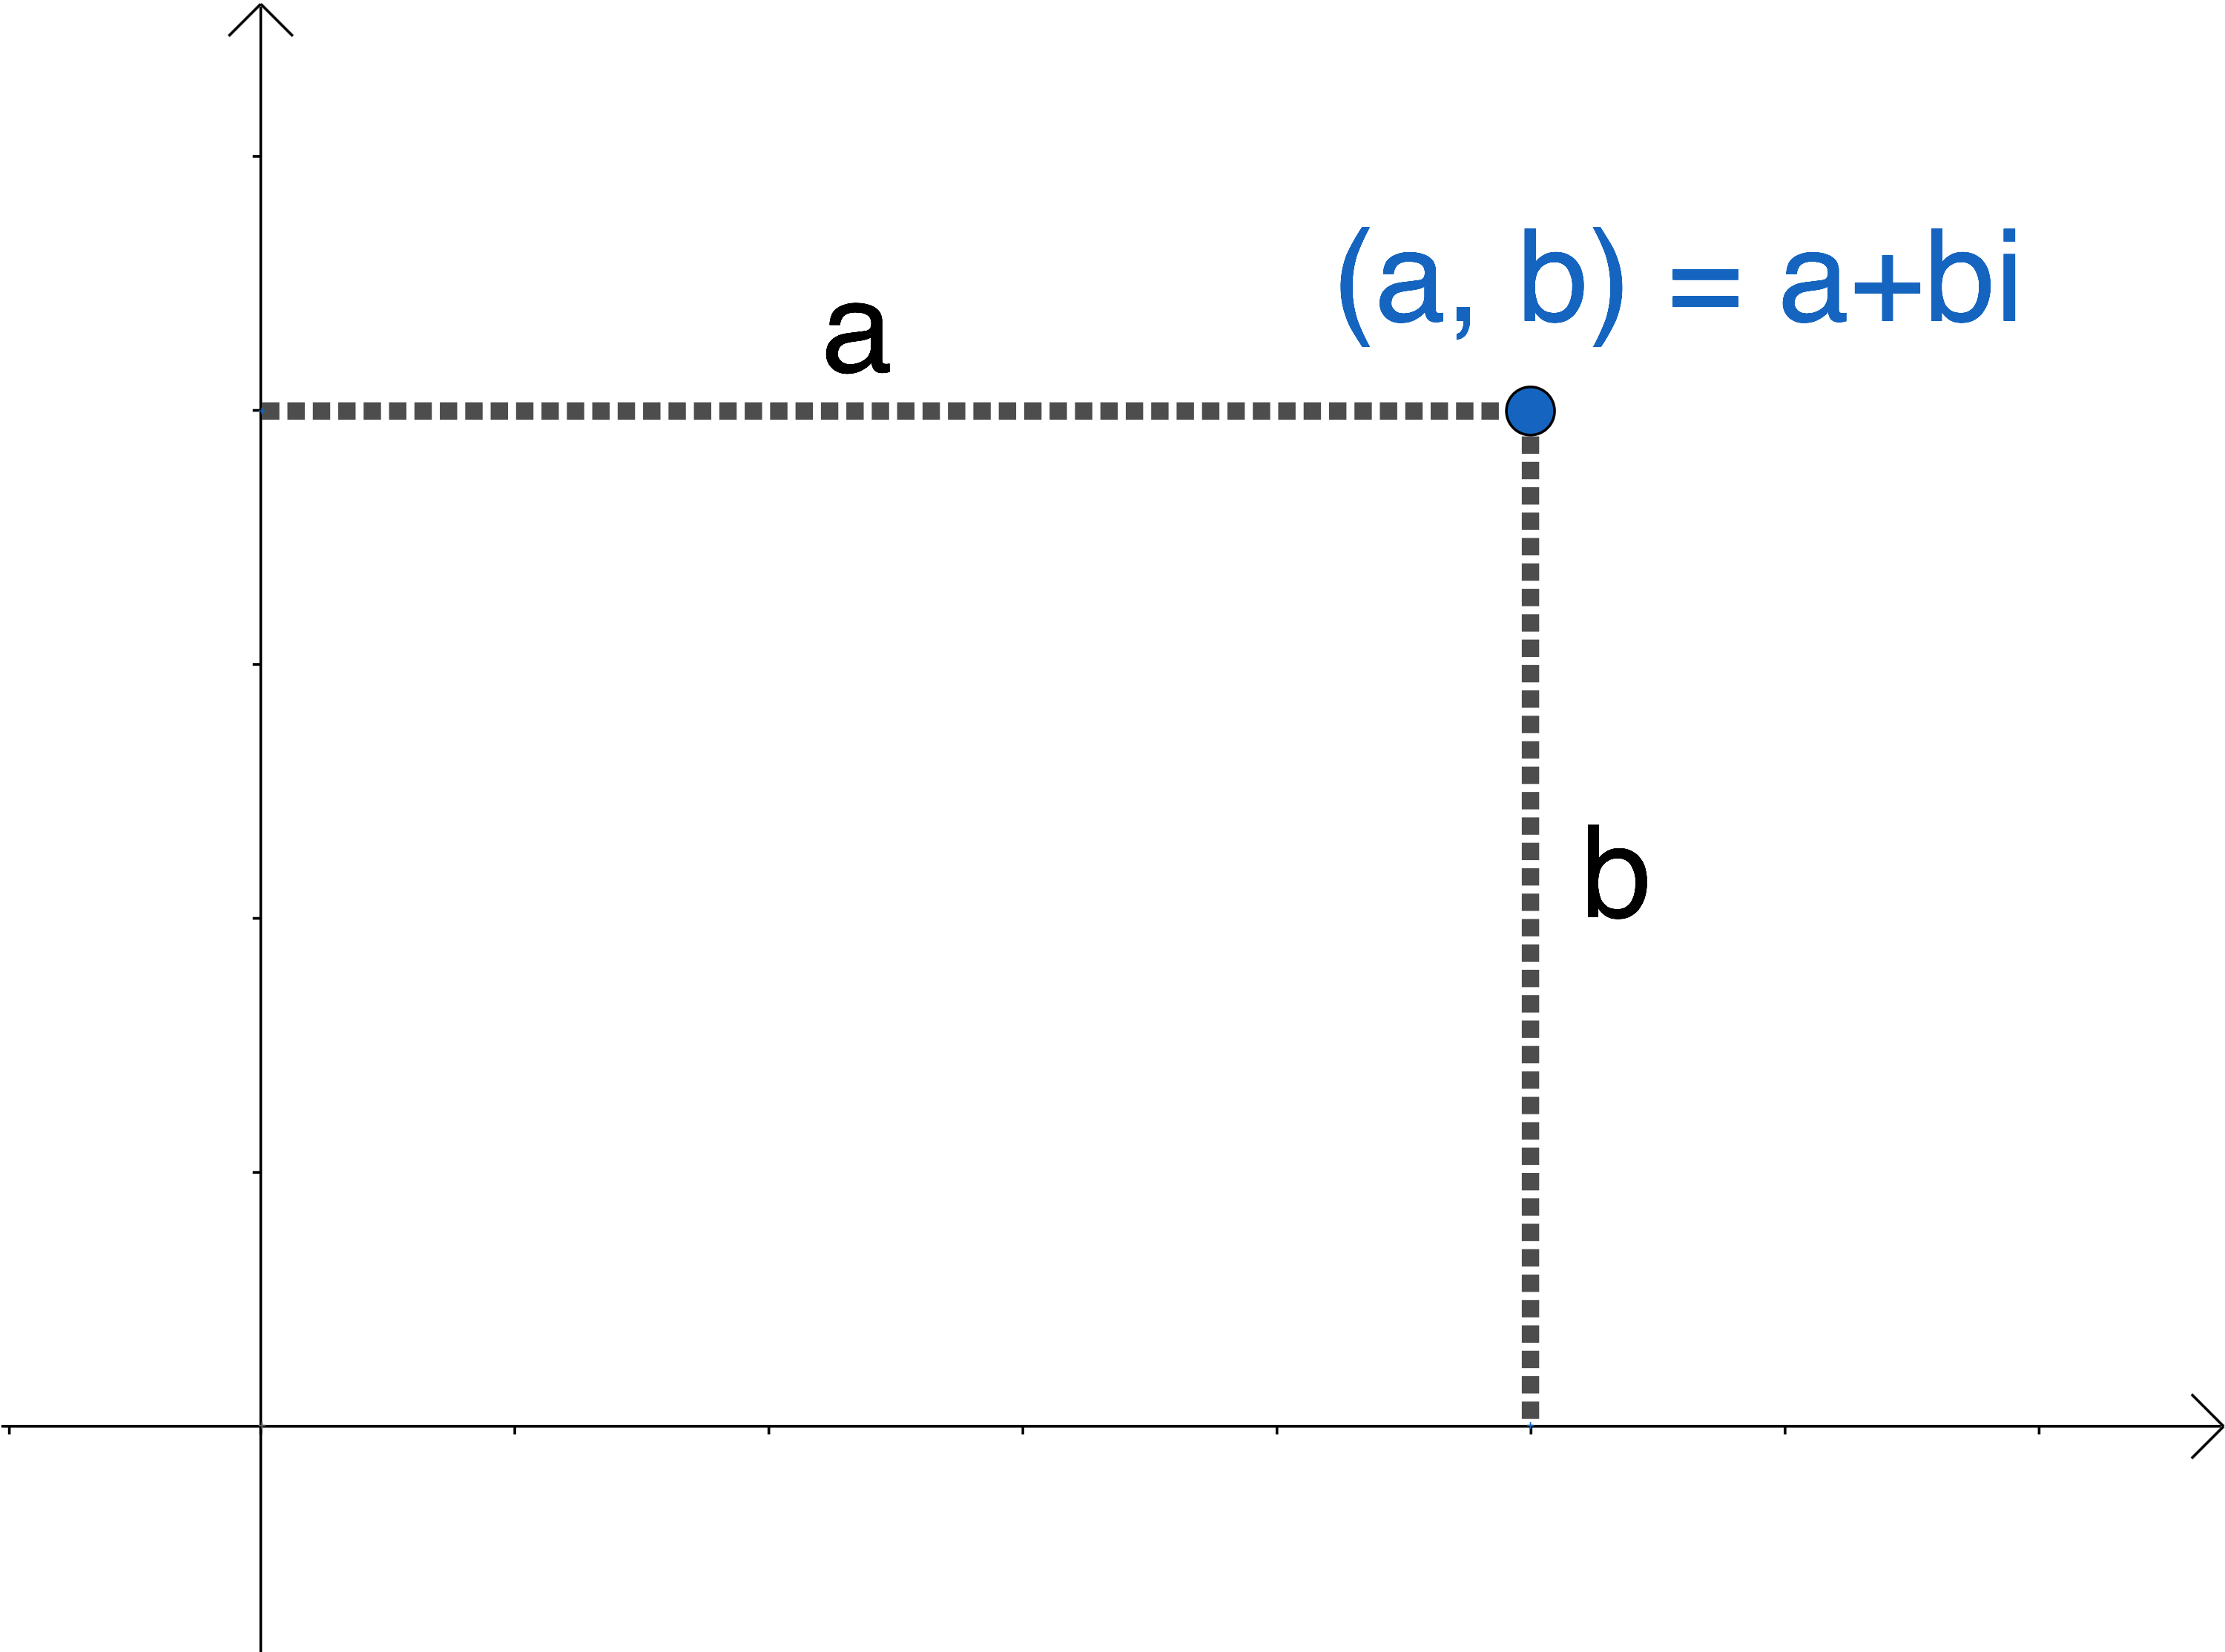
\includegraphics{complex-plane.png}
\end{frame}

\begin{frame}{Addition of complex numbers}
\begin{columns}
\column{0.4\textwidth}
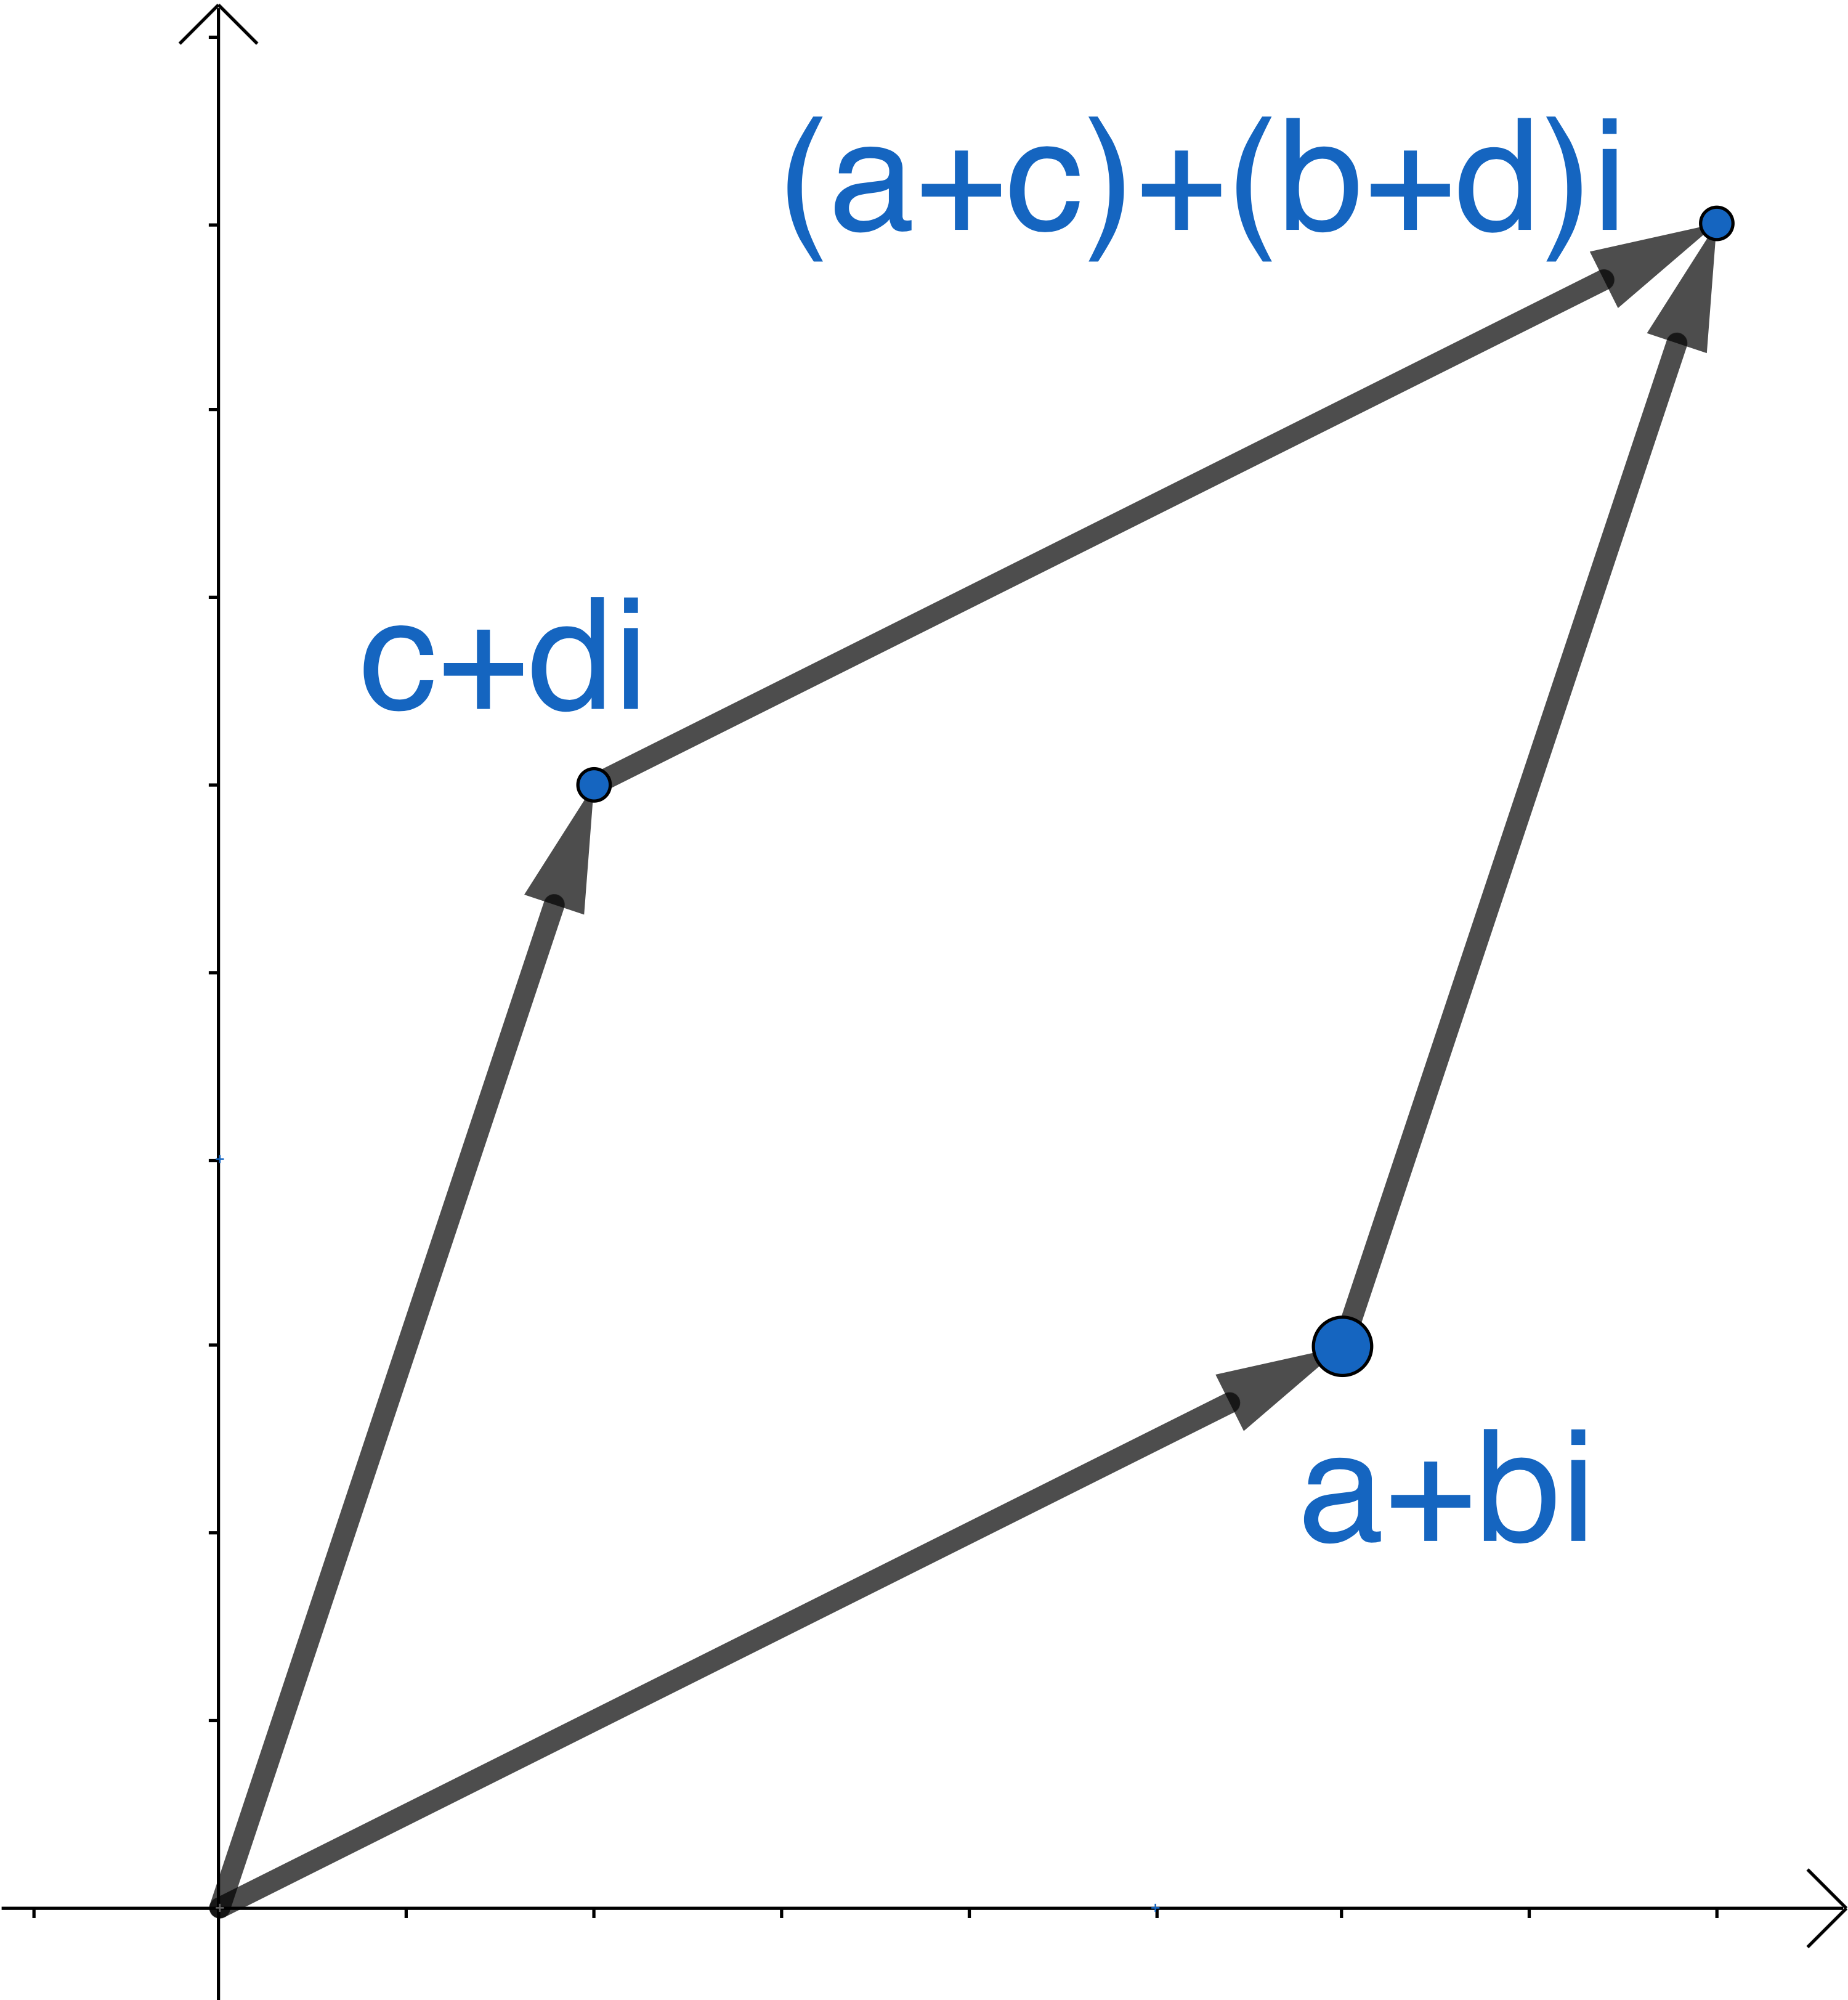
\includegraphics[scale=0.5]{complex-addition.png}
\column{0.5\textwidth}
Complex addition is defined component-wise:
\begin{equation*}
(a+ib)+(c+id) = (a+c)+(b+d)i
\end{equation*}
and therefore has the same graphical interpretation as the addition of vectors in $\mathbb{R}^2$.
\end{columns}
\end{frame}

\begin{frame}{Examples}
\begin{example}
Evaluate
\begin{itemize}
\item $(-3+6i) + (5-i)$.
% Ans: 2+5i
\item $(4-7i) + (6-2i)$.
% 10-9i
\item $(-3+6i) - (5-i)$.
%-8+7i
\item $(4-7i) - (6-2i)$.
%-2-5i
\end{itemize}
\end{example}
\begin{example}
\begin{equation*} 
(2-3i)(-3+4i) 
\end{equation*}
% ANS: 6+17i
\end{example}
\end{frame}

\begin{frame}{Historical curiosity}
Apparently Bombelli describes complex arithmetic thus:
\begin{quote}
"Plus by plus of minus, makes plus of minus.
Minus by plus of minus, makes minus of minus.
Plus by minus of minus, makes minus of minus.
Minus by minus of minus, makes plus of minus.
Plus of minus by plus of minus, makes minus.
Plus of minus by minus of minus, makes plus.
Minus of minus by plus of minus, makes plus.
Minus of minus by minus of minus makes minus." 
\end{quote}
according to Crossley in `The Emergence of Number'.
A hint from Crossley is: the last two lines would become 
\begin{equation*}
-\sqrt{-a}\cdot\sqrt{-b}= \sqrt{ab}\text{ and }(-\sqrt{-a})\cdot(-\sqrt{-b})= -\sqrt{ab}
\end{equation*}
in modern notation.
\end{frame}

\begin{frame}{Summary}
\begin{itemize}
	\item Graphical interpretation.
	\item Addition: algebra and geometry.
	\item Multiplication: algebra and geometry.
	\item Conjugate: algebra and geometry.
\end{itemize}
\end{frame}



\begin{frame}{Examples}
\begin{example}
Find all complex numbers $z$ such that $z^2 = -3+4i$.
%% Ans: z = 1+2i or z = -1-2i
\end{example}
\begin{example}
\begin{itemize}
\item If $z=3+4i$, then $\overline{z}= 3-4i$,
i.e., $\overline{3+4i}=3-4i$.
\item $\overline{-2+5i}= -2-5i$.
\item $\overline{i}= -i$.
\item $\overline{7}= 7$.
\end{itemize}
\end{example}
\end{frame}

\begin{frame}{Clearing denominators}
\begin{example}[Exemplar]
Write 
\begin{equation*}
\frac{a+bi}{c+di}
\end{equation*}
in the form $e+fi$ for real numbers $a$, $b$, $c$, $d$, $e$, and $f$.
\end{example}
\begin{itemize}
\item $\frac{1}{i}$ % ANS -i
\item $\frac{2-i}{3+4i}$ % ANS 2/25 -(11/25)i
\item $\frac{1-2i}{-2+5i}$ % ANS -(12/29) -(1/29)i
\end{itemize}
\end{frame}
% Stopped at page 17 of first set of slides.


\end{document}